\documentclass[UTF8,12pt, AutoFakeBold,fontset = founder]{ctexart}
% fontset = founder 设置更加丰富的字体
\usepackage{geometry,amsmath,amsthm,amssymb,amsfonts}
\usepackage{graphicx}
\usepackage{float}  % 导入代码块浮点包
\usepackage{microtype} % 解决行溢出问题
\setlength{\emergencystretch}{3em} % 解决行溢出问题


% \setlength{\voffset}{0.6cm} % 将页面内容向上移动

\usepackage{fancyhdr}
\renewcommand{\headrulewidth}{0pt} % 移除页眉横线
% \sectionfont{\centering} % 居中显示标题
\fancyhf{} % 清空当前的页眉和页脚设置
\fancyfoot[C]{\thepage} % 将页码放置在页脚中央

% 定义自定义的页眉页脚样式
% \fancypagestyle{plain}{ % 'plain' 是文档类默认的页面样式
%   \fancyhf{}  % 清空默认的页眉页脚
%   \fancyfoot[C]{\thepage}  % 页脚居中显示页码
% }

\usepackage{sectsty}
\usepackage{authblk} % 对应中文部分的作者机构特殊语法
\usepackage{booktabs}
\usepackage{enumitem}

\usepackage{titletoc}
\usepackage{titlesec}
\usepackage{zhnumber} % 设置标题中文序号
\renewcommand\thesection{\zhnum{section}}
\renewcommand\thesubsection{\arabic{section}.\arabic{subsection}}

\usepackage{tocloft} % 用于定制目录中的条目格式

% 重定义目录标题
\renewcommand{\contentsname}{%
  \fontsize{16pt}{24pt}\selectfont % 三号字体,1.5 倍行距
  \bfseries 目录 % 加粗
  \vspace{24pt} % 段前 24 磅
}

% % 设置目录中章节标题的格式
% \titlecontents{section}
%   [0em] % 左边距
%   {\bfseries \songti \fontsize{11pt}{13pt}\selectfont} % 标题格式
%   {\contentslabel{0.9em}{、}} % 标签格式(序号和顿号)
%   {}
%   {\titlerule*{.}\contentspage}

% % 设置目录中二级标题格式
% \titleformat{\subsection}
%   {\songti \fontsize{12pt}{18pt}\selectfont} % 宋体、小四号
%   {\thesubsection} % 编号
%   {0em} % 编号与标题之间的水平间距
%   {} % 标题内容前的附加内容
%   [\vspace{0pt}] % 段后 0 磅

% % 设置目录中三级标题格式
% \titleformat{\subsubsection}
%   {\songti \fontsize{12pt}{18pt}\selectfont} % 宋体、小四号
%   {\thesubsubsection} % 编号
%   {0em} % 编号与标题之间的水平间距
%   {} % 标题内容前的附加内容
%   [\vspace{0pt}] % 段后  0 磅


  \CTEXsetup[name={第,章},number={{\arabic{section}}}]{section}
  \sectionfont{\centering} % 居中显示标题

% 使用 titlesec 设置章节与标题的分隔符
\titleformat{\section}
  {\bfseries \heiti \fontsize{14pt}{21pt}\selectfont} % 字体设置
  {\thesection} % 编号
  {0em} % 编号与标题之间的水平间距
  {、} % 标题内容前的附加内容
  [\vspace{0.5em}] % 标题后的垂直间距

% 设置 subsection 格式
\titleformat{\subsection}
  {\mdseries \heiti \fontsize{12pt}{18pt}\selectfont} % 黑体、小四号、加粗
  {\thesubsection} % 编号
  {1em} % 编号与标题之间的水平间距
  {} % 标题内容前的附加内容
%   [\vspace{0.5em}] % 标题后的垂直间距

% 设置 subsubsection 格式
\titleformat{\subsubsection}
  {\mdseries \heiti \fontsize{12pt}{18pt}\selectfont} % 黑体、小四号、加粗
  {\thesubsubsection} % 编号
  {1em} % 编号与标题之间的水平间距
  {} % 标题内容前的附加内容
%   [\vspace{0.5em}] % 标题后的垂直间距

\usepackage[numbers,sort&compress]{natbib}

% \CTEXsetup[name={\heiti \fontsize{14.4pt}{21pt}\selectfont},number={}]{section}

% \CTEXsetup[format={\Large\bfseries}]{section}

\setlength{\baselineskip}{20pt}  % 正文20磅行距

\usepackage{listings} % 配置附件代码块
\usepackage{setspace}
\usepackage{ragged2e} % 设置两端对齐需要的模块
\newcommand{\sectspacemode}{\setstretch{1.5}} % 设置\section内容的行距为1.5倍

\usepackage{hyperref} % 点击跳转
\usepackage{xcolor} % 引入颜色包
\usepackage{caption}
\usepackage{subcaption} % 引入子图
\usepackage{extsizes} % 扩展字体,允许使用字号更大

\hypersetup{hidelinks,
	colorlinks=true,
	linkcolor=black,  % 目录链接的颜色
    citecolor=blue,  % 文献引用的链接颜色
	pdfstartview=Fit,
	breaklinks=true
}

%! 下面这条命令是不压缩pdf, 这样编译tex会很快,但是最终的pdf会很大,如果最终定稿了,请注释掉此行,这样最终的pdf会更小
\special{dvipdfmx:config z 0}

% 设置图、表、公式
\counterwithin{figure}{section}
\renewcommand{\figurename}{Figure} % 将图变成figure
\counterwithin{table}{section}
\renewcommand{\tablename}{Table}
\counterwithin{equation}{section}

\renewcommand{\thefigure}{\arabic{section}.\arabic{figure}}
\renewcommand {\thetable} {\arabic{section}.\arabic{table}}
\renewcommand {\theequation} {\arabic{section}.\arabic{equation}}

\captionsetup{labelformat=default,labelsep=space} %去除图注、表注的冒号
% 设置图像图注为中文
\captionsetup[figure]{name=图}
% 设置表格图注为中文
\captionsetup[table]{name=表}

% 作者格式
% \renewcommand*{\Authsep}{,}
% \renewcommand*{\Authand}{,}
% \renewcommand*{\Authands}{,}

\geometry{paperwidth=21cm, paperheight=29.7cm,left=3cm,right=3cm,top=2.5cm, bottom=2.5cm}

% 设置中文字体为宋体
\setCJKmainfont{SimSun}

% 设置英文字体为 Times New Roman
\setmainfont{Times New Roman}
% 引入华文行楷字体
\setCJKfamilyfont{huawenxingkai}{STXingkai} % 字体名称可能与系统显示不同,需确认
\newcommand{\huawenxingkai}{\CJKfamily{huawenxingkai}}

% 设置段落格式
\setlength{\parindent}{2em} % 首行缩进 2 字符
\setlength{\parskip}{0pt} % 段前段后 0 磅
\linespread{1.08} % 行距 20 磅(12pt × 1.08 ≈ 20pt)
\justifying % 两端对齐

% \title{Prediction of urban air quality by data mining}
% % authblk 提供的特殊用法,将作者机构作为 option 进行捆绑
% \author[1]{Long Liu}
% \affil{School of Information Engineering}
% \date{}

\begin{document}
% \begin{sloppypar}
\makeatletter
% 定义引用格式
\def\@cite#1#2{\textsuperscript{[{#1\if@tempswa , #2\fi}]}}
\setlist[enumerate]{itemsep=0pt, parsep=0pt} % 设置enumerate环境的垂直间距

\makeatletter 
{
    \thispagestyle{empty}
    \begin{center}
        \includegraphics[height=2.07cm, width=10.03cm]{../images/school.png}
        \vspace*{1\baselineskip}\\
        {\fontsize{36}{43.2}\selectfont{\huawenxingkai 硕\ 士\ 学\ 位\ 论\ 文}}\\
        \vspace*{4.6\baselineskip}
        {\fontsize{24}{28.8}\selectfont\heiti 题\ \ \ 目}
        \vspace*{1\baselineskip}\\
        {\fontsize{24}{28.8} \underline{\heiti{基于图像分割的细粒度变形表格结构识别}}}
    \end{center}
    \vspace*{3\baselineskip}
    \begin{center}
    \begin{table}[!htbp]
    \centering
        \begin{tabular}{c @{\hspace{2cm}} c rc}
            \Large \makebox[3cm][s]{\fontsize{15pt}{15pt}\selectfont \textbf{\songti 学号:}}&{\makebox[5cm][l]{\fontsize{15pt}{15pt}\selectfont \textbf{2304081200008}}} \\
            \\[1pt]
            \Large \makebox[3cm][s]{\fontsize{15pt}{15pt}\selectfont \textbf{\songti 硕士研究生:}}&{\makebox[5cm][l]{\fontsize{15pt}{15pt}\selectfont \textbf{刘龙}}} \\
            \\[1pt]
            \Large \makebox[3cm][s]{\fontsize{15pt}{15pt}\selectfont \textbf{\songti 指导教师:}}& {\makebox[5cm][l]{\fontsize{15pt}{15pt}\selectfont \textbf{杨词慧副教授}}} \\
            \\[1pt]
            \Large \makebox[3cm][s]{\fontsize{15pt}{15pt}\selectfont \textbf{\songti 学院:}}&{\makebox[5cm][l]{\fontsize{15pt}{15pt}\selectfont \textbf{信息工程学院}}} \\
            \\[1pt]
            \Large \makebox[3cm][s]{\fontsize{15pt}{15pt}\selectfont \textbf{\songti 专业:}}& {\makebox[5cm][l]{\fontsize{15pt}{15pt}\selectfont \textbf{计算机科学与技术}}} \\
            \\[1pt]
            \Large \makebox[3cm][s]{\fontsize{15pt}{15pt}\selectfont \textbf{\songti 研究方向:}}& {\makebox[5cm][l]{\fontsize{15pt}{15pt}\selectfont \textbf{计算机视觉}}} \\
            \\[1pt]
            \Large \makebox[3cm][s]{\fontsize{15pt}{15pt}\selectfont \textbf{\songti 日期:}}& {\makebox[5cm][l]{\fontsize{15pt}{15pt}\selectfont \textbf{2024年12月}}}
        \end{tabular}
    \end{table} 
    \end{center}

\begin{center}
    \vspace*{\baselineskip}
    {\Large \fangsong 南昌航空大学研究生院制}
\end{center}
% \vspace{-2\baselineskip} % 减少一定的空间
\restoregeometry
}

{
    \thispagestyle{empty}
    \begin{center}
        \includegraphics[height=2.07cm, width=10.03cm]{../images/school.png}
        \vspace*{1\baselineskip}
        \newline
        {\fontsize{36}{43.2}\selectfont{\huawenxingkai 硕\ 士\ 学\ 位\ 论\ 文}}\\
        \vspace*{4.6\baselineskip}
        {\fontsize{21pt}{21pt} \textbf{\songti{基于图像分割的细粒度变形表格结构识别}}}
    \end{center}
    \vspace*{3\baselineskip}
    \begin{center}
    \begin{table}[!htbp]
    \centering
        \begin{tabular}{c @{\hspace{2cm}} c rc}
            \Large \makebox[3cm][s]{\fontsize{15pt}{15pt}\selectfont \textbf{\songti 学号:}}&{\makebox[5cm][l]{\fontsize{15pt}{15pt}\selectfont \textbf{2304081200008}}} \\
            \\[1pt]
            \Large \makebox[3cm][s]{\fontsize{15pt}{15pt}\selectfont \textbf{\songti 硕士研究生:}}&{\makebox[5cm][l]{\fontsize{15pt}{15pt}\selectfont \textbf{刘龙}}} \\
            \\[1pt]
            \Large \makebox[3cm][s]{\fontsize{15pt}{15pt}\selectfont \textbf{\songti 指导教师:}}& {\makebox[5cm][l]{\fontsize{15pt}{15pt}\selectfont \textbf{杨词慧副教授}}} \\
            \\[1pt]
            \Large \makebox[3cm][s]{\fontsize{15pt}{15pt}\selectfont \textbf{\songti 学院:}}&{\makebox[5cm][l]{\fontsize{15pt}{15pt}\selectfont \textbf{信息工程学院}}} \\
            \\[1pt]
            \Large \makebox[3cm][s]{\fontsize{15pt}{15pt}\selectfont \textbf{\songti 专业:}}& {\makebox[5cm][l]{\fontsize{15pt}{15pt}\selectfont \textbf{计算机科学与技术}}} \\
            \\[1pt]
            \Large \makebox[3cm][s]{\fontsize{15pt}{15pt}\selectfont \textbf{\songti 研究方向:}}& {\makebox[5cm][l]{\fontsize{15pt}{15pt}\selectfont \textbf{计算机视觉}}} \\
            \\[1pt]
            \Large \makebox[3cm][s]{\fontsize{15pt}{15pt}\selectfont \textbf{\songti 日期:}}& {\makebox[5cm][l]{\fontsize{15pt}{15pt}\selectfont \textbf{2024年12月}}}
        \end{tabular}
    \end{table} 
    \end{center}

\begin{center}
    \vspace*{\baselineskip}
    {\Large \fangsong 南昌航空大学研究生院制}
\end{center}
% \vspace{-2\baselineskip} % 减少一定的空间
\restoregeometry
}

\makeatother

\pagestyle{fancy} % 从这个地方一下全遵循自定义页眉
\newpage
% 添加目录
% 设置目录的独立页码
\pagenumbering{Roman} % 使用小写罗马数字作为目录页码
\setcounter{page}{1} % 重置页码计数器
\begin{flushleft}
    \centering\tableofcontents
\end{flushleft}


\clearpage

% {
%     \pagenumbering{Roman}
%     \thispagestyle{plain}
%     % \maketitle
%     \rhead{Abstract}
%     \begin{center}
%         \section*{\centerline{Abstract}}
%     \end{center}

%     This paper mainly studies the problem of urban air quality, and establishes a model based on \textbf{typical correlation analysis} and neural network algorithm to predict air quality,This article measures the air quality specifically refers to the occurrence of haze.

%     In this paper, After data acquisition, statistical software SPSS26 was used for typical correlation analysis, and three typical correlation coefficients were selected and standardized from the correlation coefficient and typical correlation degree. At the same time, the typical load is introduced to describe the index of each typical correlation coefficient reaction. Finally, the contribution of the typical variables to the total variance of the sample is described. The proportion of variance explained by the three typical variables is 0.365, 0.203 and 0.031, respectively.

%     Considering that the forecast is not stable and needs to be updated with time, this paper does not consider meteorological conditions and seasonal factors with a long time span. In terms of method, this paper considers to build \textbf{BP neural network algorithm} with matlab, and adopts \textbf{Levenberg-Marquardt training algorithm} to build model prediction. Finally, when the fit degree allows, the model can indirectly obtain the corresponding PM2.5 through weather forecast data The predicted value can be combined with the haze level warning to predict the air quality.
%     \newline 
%     \vspace*{0.3\baselineskip}
%     \medskip\textbf{【Keywords】}typical correlation analysis;BP neural network algorithm;Levenberg-Marquardt training algorithm
%     \clearpage
% }
% \pagenumbering{arabic}

\pagenumbering{arabic} % 切换到阿拉伯数字作为正文页码
\setcounter{page}{1} % 重置页码计数器
% 通常来说,你在下面章节填充内容即可!
\section{选题依据}

\subsection{研究背景}

在信息化的时代,随着扫描、拍照等手段的普及以及大数据和人工智能的推动,纸质文档逐渐被电子文档取代。传统的纸质文档多依赖人工输入和手动整理,需要消耗大量人力资源与时间成本,而电子文档则得益于计算机技术的发展,能自动存储、编辑及检索,极大提升了信息处理之效率与准确性。

表格中不仅包含文字信息,还包含复杂的行列关系、合并单元格以及多种对齐方式等,这些因素使得光学字符识别(OCR)\cite{b1, b2}技术在提取表格数据时面临不小的挑战。比如在一些复杂表格中,虽然OCR能够识别出单元格中的文本内容,但难以准确推断出单元格之间的层级关系和从属结构,这在一定程度上限制了其在表格数据提取中的应用。

为了应对文档中复杂表格结构的解析需求,准确获取获取表格中的行列关系、单元格合并、对齐方式等特性,研究者们开始探索表格结构识别方法,表格结构识别指的是从文档图像中自动提取表格的布局信息,并重建其行列关系。一个标准的表格由若干行列组成,当前,表格结构识别的研究方法主要可以分为两类:基于规则的传统方法和基于深度学习的现代方法。基于规则的传统方法通常依赖于图像处理技术,例如边缘检测、投影分析、连通域分析等\cite{b3}。这些方法通过寻找表格的行列线条来判断结构,但在实际应用中,表格往往存在复杂的合并单元格、倾斜、扭曲等形变,这些都使得基于线条的传统方法效果不佳。因此,很多新方法开始尝试不依赖明确的线条,而是通过单元格的定位来重建表格结构。通过定位单元格的起始和结束位置,可以有效避免线条缺失或干扰的影响,从而实现对复杂表格的识别。

近年来,深度学习方法在表格结构识别中的应用取得了突破性进展\cite{b3}。深度学习模型尤其是卷积神经网络(CNN)在图像分割与特征提取方面展现了巨大的优势。对于表格结构的识别,部分基于深度学习的方法依然采用了线条检测来恢复表格的行列结构,例如通过检测图像中的水平和垂直线条来推测行列划分。这类方法通常能够应对大多数标准表格,但对于复杂的表格(如包含合并单元格或倾斜表格),识别效果却并不理想。而另外一些方法则不直接依赖于线条,而是通过单元格区域的检测和定位来判断表格的结构\cite{bcell}。这类方法通常依赖于深度神经网络的端到端训练,直接从图像中学习表格的布局和结构,并能自动进行表格的恢复和数据提取。

如今,表格图像的结构识别依然面临诸多难题。首先,表格的多样性和复杂性对识别提出了严峻挑战。现代文档中的表格形式多样,不仅包括基本的网格结构,还可能包含合并单元格、斜线分隔符、嵌套表格等复杂形式,传统表格识别算法往往难以处理。此外,形变表格的出现进一步增加了识别难度。例如,由于扫描角度的变化或内容被拉伸、倾斜等原因,表格图像可能出现变形,导致传统识别方法无法准确提取结构信息。尤其是表格中的单元格划分和内容对齐,在图像形变或变形后容易发生偏移,这使得表格的检测和重建变得更为复杂。因此,如何高效、准确地识别和重建表格结构,已成为亟待解决的难题。

\subsection{研究意义与目的}

在文档存储数据的方式中,表格占据着举足轻重的地位,尤其是在财务报表、学术论文、统计分析等领域,它们不仅是信息传递的重要载体,也是数据分析的基础。因此,从图像文档中自动提取表格信息并重建其结构的过程,逐渐成为计算机视觉和图像处理领域备受关注的研究方向。这项工作的核心挑战在于如何高效且准确地从复杂的图像背景中分离出表格区域,识别表格内部的行列布局,并进一步精准提取每个单元格内的数据内容。这不仅有助于提升信息处理的自动化水平,减少人工干预所带来的误差,同时也为后续的数据分析提供了更加可靠的支持。此外,随着移动设备和数字化办公环境的普及,能够快速准确地处理各种形式存在的表格图像,对于促进跨平台的信息共享与交流也具有重要意义。

\section{国内外研究现状}

由于表格的形式多样且版面不固定,且常常受到印章、褶皱等因素的影响,表格识别仍然面临着许多挑战。为了解决这些问题,国内外的研究机构和学者进行了大量的研究,探索了多种方法。为了更好地总结前人工作的成果,并为后续研究提供参考,本节将从表格区域检测、表格结构识别和端到端表格识别技术三个方面介绍该研究方向的发展历程和最新研究进展,旨在全面展示该领域的技术演进和当前的研究趋势。

\subsection{表格区域检测}

作为表格结构识别的前提,表格区域识别的研究目标是从文档中准确定位出表格的所在区域,经过了启发式方法、机器学习方法,再到深度学习方法的逐步演变。早期的表格区域识别主要依赖于启发式或规则方法。这类方法基于视觉特征,例如字符对齐、行间间隔、文本块的布局结构,甚至结合文本信息,通过手工设计的规则来识别表格区域。例如,Pyreddy\cite{m1}等人通过字符对齐、孔和间隔来检测表格;Jahan 等人基于字间距和行高的局部阈值来定位表格区域。这些启发式方法在文档布局统一或格式较简单的情况下效果良好,但在处理复杂的表格布局(例如嵌套表格、多列表格等)或不同布局的文档时,往往需要调整规则,通用性较差。为了提高这类方法的适应性,后续研究提出了更多复杂的规则设计。例如,Nurminen 等人提出了一种通过共同对齐方式来定位文本框的启发式方法,并为每个文本框分配成为表格的概率。这类方法相对更适应格式多变的表格,但其检测精度依旧受限于规则设计的复杂性,尤其在大型文档处理任务中效率较低。

随着机器学习技术的快速发展,表格区域识别逐步转向基于机器学习的研究方向。相比于启发式方法,机器学习方法通过数据驱动模型,从训练数据中自动学习特征,大大减少了手工规则的设计。例如,Kieninger\cite{m3}等人使用无监督的聚类方法对表格区域进行识别,通过自动聚类分词来提升表格识别的效果;Cesarini\cite{m4}等人则提出改进的 XY 树结构方法,通过监督学习来检测文档中的表格。Fan\cite{m5}等人在 PDF 文件中使用了监督和非监督方法相结合的策略以提高表格区域检测的稳定性和准确性。此外,Wang\cite{m2}等人将决策树和 SVM 分类器应用于文档的布局和内容特征,以实现更具适应性的表格检测。然而,尽管机器学习方法在模型泛化性上有所提高,其效果仍依赖于特定特征的设计和特定类型数据的训练,在处理文档样式多变的情况下模型的表现仍有局限。

近年来,随着深度学习技术的广泛应用,表格区域识别迎来了新的研究范式。深度学习通过构建深层神经网络,能够自动提取特征并学习更为复杂的模式,显著提升了表格区域识别的准确性和适应性。在表格区域识别中,目标检测和语义分割方法是常用的两类技术。目标检测方法将表格视为检测目标,利用卷积神经网络(CNN)识别并标注出表格区域。例如,Hao 等人使用 R-CNN 进行表格检测,Madhav Agarwal\cite{m13}等人则采用 Mask R-CNN 技术提升了表格区域检测的精度。另一方面,语义分割方法将文档图像划分为不同的语义类别(如表格区域、文本区域),实现了对复杂布局的细粒度识别。例如,Yang\cite{m11}等人提出的多尺度全卷积网络在对不同大小和形状的表格区域检测方面具有良好表现。通过深度学习模型的自适应学习特性,表格区域识别的通用性显著提升,能够更好地处理复杂布局的文档,尤其在包含多样化表格格式的大规模文档数据中展现出较强的泛化能力。

\subsection{表格结构识别}

表格结构识别的研究目标是在定位表格区域的基础上,进一步识别表格内部的结构信息,例如行、列、单元格和表头等结构元素。这一方向的研究经历了启发式方法、机器学习方法,再到深度学习方法的发展历程。在表格结构识别早期,研究者主要依靠启发式规则来分解表格的结构信息。这类方法依赖于文本块的排列、表格线的分布等信息,通过手工设计的规则来实现。例如,Chandran\cite{m24}等人提出通过垂直线和水平线的交叉来检测表格结构;Hassan\cite{m25}等人通过分析文本块的空间特征来定位和分割表格结构。此外,Ruffolo\cite{m26}等人开发了 PDF-trex 系统,通过页面元素的空间特征进行表格结构识别。这类方法在特定的表格格式中具有较高的准确性,但对于复杂表格的识别效果仍不理想,且缺乏足够的灵活性以应对多样化的文档结构。

机器学习方法的引入为表格结构识别带来了新的可能性。通过学习表格结构的特征分布,机器学习方法能够在一定程度上提升识别的准确性。Kieninger\cite{m3}等人采用了无监督的聚类分词学习方法来识别表格结构;Silva 等人使用隐马尔可夫模型将潜在的表行合并为表结构;Kasar 等人则基于支持向量机(SVM)对文本区域进行分类,从而实现表格结构的识别。这些方法虽然提高了模型的通用性,但依旧面临复杂表格结构识别的瓶颈,例如多层嵌套表格、无边框表格等场景。

在深度学习方法的推动下,表格结构识别取得了显著的进展。深度学习模型如 CNN、RNN、图神经网络(GNN)等,能够自动学习结构特征,显著提高了表格结构识别的精度和适应性。当前的研究主要分为目标检测、语义分割、图模型和图像到标记序列几种方法。目标检测方法通过将表格结构分解为行、列、单元格等元素来实现结构识别。例如,Siddiqui\cite{m21}等人提出的 DeepTabStR模型和 R.Long\cite{m22}等人提出的 Cycle-CenterNet 模型都在表格结构分解上取得了良好效果。语义分割方法则将表格图像划分为不同的语义类别(如单元格、行、列、标题等),例如 Schreiber\cite{m12}等人提出的 DeepdeSRT 模型和 Paliwal\cite{m17}等人提出的 TableNet 模型。图模型方法进一步将表格结构表示为图形,通过图神经网络(GNN)来进行结构识别,Koci\cite{m7}等人提出的 RAC 模型和 Chi\cite{m8}等人提出的 GraphTSR 模型都是其中的代表。此外,图像到标记序列的方法受到自然语言处理的启发,将表格结构识别视为序列生成任务,通过 Transformer 等模型实现结构的序列化标记,例如Deng Y\cite{m10}等人提出的EDD模型、Ahmed Nassar\cite{m8}等人提出的TableFormer模型以及Hangdi Xing\cite{m23}等人提出的LORE模型;EDD模型过注意力编码器-解码器 (EDD) 架构,能够更好地关注图像中的关键信息,例如表格标题、单元格内容等,从而提高识别精度,TableFormer 网络使用 Transformer 解码器代替了 EDD 网络中的 LSTM 解码器,能够更好地处理长距离依赖关系,并提高识别精度。LORE模型则为表格结构识别提出了另一种范式,将表格结构识别作为一个逻辑位置回归问题,首次将逻辑回归和表格结构识别结合起来。这些方法不仅在表格结构识别的精度上实现了显著提升,同时在处理复杂的、多样化的表格结构时展现出更高的泛化能力。

总之,表格结构识别的研究发展反映了表格识别领域从简单规则到复杂模型的进步。虽然启发式和机器学习方法仍在特定场景下发挥作用,但深度学习方法因其自适应的特性,已经成为该领域的主流方向。深度学习模型在处理复杂表格和多样化文档布局时具有显著优势,这不仅提高了表格结构识别的准确性,也拓展了其在实际应用中的适用性。

\subsection{端到端的表格识别方法}

近年来,表格识别技术的研究逐步从单一的表格区域检测或结构识别任务向更为集成化的方向发展,端到端方法和以数据为中心的方法应运而生。这些方法在表格区域检测和结构识别的基础上,将两者合并为一个整体,通过单一模型实现端到端处理,从而进一步提高了识别效率和模型的适应性。在传统方法中,表格区域检测和结构识别通常作为两个独立步骤分别进行,彼此之间的交互有限。而端到端方法通过一体化设计,能够在减少手工干预的情况下自动完成表格的全面识别,显著提升了模型的效率与准确性。

端到端方法主要通过深度学习模型将表格区域检测和结构识别整合在一个流程内,实现从表格定位到结构解析的无缝衔接。这类方法的早期代表包括Sebastian Schreiber\cite{m12}等人提出的DeepDeSRT,它使用 Faster R-CNN 直接对表格进行检测和结构解析,不依赖启发式规则或元数据。后续的Madhav Agarwal\cite{m13}等人提出的CDeC-Net 则在 Mask R-CNN 的基础上增加了多级扩展,并通过可变形卷积适应不同尺度的表格布局,提升了高 IoU 阈值下的检测精度。此外,W Xue\cite{m14}等人提出的ReS2TIM 模型通过构建表格单元间的关系图并进行结构化推断,实现了从表格图像到结构表示的转换;而C Tensmeyer\cite{m15}等人提出的SPLERGE模型则通过扩张卷积建立表格网格布局,进而识别跨行或跨列的复杂单元格,进一步拓展了端到端方法对复杂表格的适应性。

在处理多样化表格格式方面,Y Deng\cite{m16}等人提出的TABLE2LATEX、SS Paliwal\cite{m17}等人提出的TableNet 和 Devashish Prasad\cite{m18}等人提出的CascadeTabNet 的一系列端到端模型表现出了出色的性能。TABLE2LATEX 通过将表格图像与 LaTeX 源代码配对,利用注意力编码器-解码器模型直接生成 LaTeX 格式的结构化输出,这种设计有效地解决了表格识别到格式化表示的转化问题。TableNet 在训练过程中增加了空间语义的关联,使得表格检测和结构识别两项任务之间的依赖关系得到了充分利用,进一步提升了识别精度。CascadeTabNet 则通过单一卷积网络实现区域检测和结构识别的同时处理,简化了整体流程,适合大规模文档的批量处理。

新型端到端模型如Danish Nazir\cite{m19}等人提出的HybridTabNet、Hashmi K.A\cite{m20}等人提出的CasTabDetectoRS 和Wenyuan Xue\cite{m9}等人提出的TGRNet都在表格识别的精度和效率之间进行了平衡。HybridTabNet 采用 ResNeXt-101 主干结合混合任务级联 (HTC) 方法,实现高精度的表格区域检测和结构解析;CasTabDetectoRS 使用轻量级的 ResNet-50 网络,不依赖预处理和后处理即可获得较高的识别效果;TGRNet 将表格结构识别重新定义为表格图重构任务,通过单元格检测和逻辑位置预测的双分支设计,有效解决了复杂表格的解析问题。此外,TSR-dsaw 和 WSTabNet 等模型进一步探讨了端到端识别和输出格式化的结合,通过直接生成 HTML 或 LaTeX 格式的结构化数据,实现了从图像到结构表示的端到端训练。Multi-Task 模型则通过共享的编码器和多个解码器,分别处理表格的结构识别、单元格检测和内容识别等子任务,在多任务学习中展现了独特优势。总体来看,端到端方法为表格识别提供了集成化的解决方案,使得表格区域检测和结构识别可以在统一框架下完成,从而极大提升了识别效率和准确性。

除了模型架构的创新,以数据为中心的方法也为表格识别的研究提供了新的思路。这类方法强调数据质量和标注一致性的重要性,认为高质量的训练数据对模型的性能具有显著影响。以数据为中心的方法通过提升数据的数量和多样性,改进标注质量和一致性,从而增强了模型的泛化能力。例如,通过数据增强技术生成不同类型的表格样本,有助于模型适应各种表格格式和布局;数据的预处理和后处理则能够标准化模型的输入和输出,提高模型的稳定性和一致性。此外,基准对齐确保了数据标注的标准性,使得模型评估结果更具参考价值和可靠性。

在数据驱动的表格识别研究中,大规模高质量的数据集建设成为关键。TABLE2LATEX 项目通过构建包含表格图像和 LaTeX 源代码的配对数据集,为表格识别的端到端训练提供了充足的数据支持。这种高质量、结构化的数据集使得模型能够更好地学习表格的布局和结构特征,有效提升了模型在不同应用场景中的泛化能力和识别精度。整体而言,以数据为中心的方法为端到端表格识别的研究提供了强大的数据支撑,进一步推动了表格识别领域的发展。

综上所述,端到端方法和以数据为中心的方法共同推动了表格识别技术的进步。端到端方法通过整合表格区域检测和结构识别,将表格识别简化为一个单一任务,提升了模型的效率与适应性;以数据为中心的方法则通过优化数据质量和标注一致性,为模型训练提供了坚实的基础。两者的结合,不仅提高了表格识别的准确率,还为应对复杂、多样化的表格数据提供了更加高效和可靠的解决方案。

% \subsection{数据集}

% 表格识别技术的发展离不开高质量数据集的支持,这些数据集为研究者提供了多样化的训练样本,推动了表格识别算法的进步。多个经典数据集为该领域提供了重要的基础。例如,UW-3\cite{data1}(1996年)数据集包含1600张经过倾斜校正的英文文档图像,奠定了表格识别的早期基础;UNLV\cite{data1}(2012年)和Marmot\cite{data1}(2012年)数据集提供了大量扫描文档图像和实体边界框,涵盖了不同类型和布局的表格;ICDAR 2013、ICDAR 2015\cite{data2}和ICDAR 2017\cite{data3}数据集作为表格识别领域的基准数据集,广泛应用于表格检测与结构识别竞赛。随着研究的深入,DeepFigures\cite{data5}(2018年)和ICDAR 2019\cite{data4}(2019年)等数据集相继发布,进一步丰富了表格识别的研究样本,支持表格检测和结构识别任务。PubTabNet\cite{data6}(2020年)和TableBank\cite{data7}(2020年)则为表格检测和结构识别提供了大量HTML格式的表格数据,推动了数据驱动的表格识别技术的发展。SciTSR\cite{data8}(2019年)和FinTab\cite{data9}(2021年)则专注于特定领域,如科学论文和财务表格,提供了多样化的标注数据。此外,WTW\cite{data10}(2021年)数据集专注于自然场景下的表格数据,特别针对图像的扭曲、倾斜等失真问题,提供了形变表格识别的重要数据支持,推动了该领域的进展。最新发布的PubTables-1M\cite{data11}(2022年)和TabRecSet\cite{data12}(2022年)数据集为端到端表格识别提供了大量样本,涵盖了多种语言和表格类型,进一步扩展了表格识别技术的应用范围。WikiTableSet\cite{data13}(2023年)包含近400万张英文、日文和法文表格图像,为跨语言的表格识别研究提供了重要的数据支持。这些数据集的发布为表格识别技术的发展提供了重要的数据支撑,推动了表格识别算法的进步,并为未来的研究提供了宝贵的资源。

\section{预期目标}

通过对本文提出的问题的研究,结合现有的表格识别方法,预期达到以下目标:

对于存在形变的有网格线表格图像,设计并实现一种基于深度学习的图像分割方法,尽最大可能识别和分割表格中每个单元格的细粒度的坐标,此外,本课题还将设计一种算法,用于确定单元格之间的相对位置,能获取单元格在表格中行、列以及合并信息。

\section{研究的主要内容}
\subsection{单元格物理坐标定位}

在表格结构识别中,单元格物理坐标用于精确描述单元格在图像中的位置,合适的单元格物理坐标的表示方法为表格结构识别提供了精确的定位基础,尤其是在表格结构重建和数据提取过程中,它们能够确保单元格位置的准确性,也为后续的单元格逻辑坐标定位提供了基础。

\subsection{基于单元格的细粒度分割模型的构建}

传统的表格结构提取方法主要依赖于线段检测和几何模型推理,这些方法虽然在处理标准化表格时表现良好,但在面对形变严重的表格时,其局限性逐渐显现。尤其是直线检测算法,通常通过霍夫变换等技术检测图像中的直线,以识别表格的行和列。尽管这种方法在结构清晰的表格中运作良好,但一旦表格因拍照或扫描产生了形变,行列的线条可能出现弯曲或断裂,从而导致算法无法有效识别,最终影响表格结构的提取精度。于是,有的研究转向通过四个关键角点来表示单元格物理坐标。

\begin{figure}[H]
    \centering
    \includegraphics[width=0.9\textwidth]{../images/point.png}
    \caption{关键点检测与图像分割}
    \label{fig:p}
\end{figure}

然而,基于关键点推理的模型也存在一定局限性,如图\ref{fig:p},单元格的边界可能形变过于严重,导致定位出得到的单元格在后期的OCR识别丢失了大量信息,也给逻辑坐标还原带来了巨大的挑战。这种情况下,单纯依靠几何形状的描述已无法满足实际需求,为了解决这些问题,本课题关注基于图像分割的技术。与关键点推理模型的方式不同,图像分割通过对图像进行像素级的处理,能够捕捉到每个单元格的边界信息,并保留更多细节。特别是在处理复杂形状和形变严重的情况下,图像分割算法展现出强大的能力,这种细粒度的识别方法能最大程度上保留单元格的内容信息区域。

\subsection{单元格逻辑坐标定位}

与单元格物理坐标不同,单元格逻辑坐标主要描述单元格之间的相对位置和从属关系,通常用于表示表格的布局结构和单元格之间的逻辑关系。通过获取单元格逻辑坐标,可以更加清楚的了解表格中单元格之间的关系,如单元格本身的行列信息、单元格的合并信息、单元格的跨行跨列信息等。这对于表格结构映射还原具有重要意义。

\subsection{表格结构映射还原}

表格重组是表格识别中的一个辅助步骤,目的是通过物理坐标和逻辑坐标的结合,将表格中的单元格从图像中的位置恢复为规整的、标准化的表格布局。这一过程帮助系统将单元格准确排列,确保不同单元格之间的空间和结构关系正确。

\section{研究方案}
\subsection{数据集的构建}

现有的形变表格数据集都是基于关键点检测或者目标识别算法,所以金标准将会不符合图像分割的需求,所以我们将采集一些形变的数据集进行,其中将会有1000张左右来自人工采集,4000张来自自然场景下的公开数据集WTW,一共5000张,然后通过人工标注,将标注结果转换为图像分割的标注格式,并使用这些数据集进行训练和测试。如图\ref{fig:label}是数据标注的掩码效果图:
\begin{figure}[H]
    \centering
    % 第一个子图
    \begin{subfigure}[b]{0.45\textwidth}
        \includegraphics[width=\textwidth]{../images/origin.png}
        \caption{原图}
        \label{fig:origin}
    \end{subfigure}
    \hfill
    % 第二个子图
    \begin{subfigure}[b]{0.45\textwidth}
        \includegraphics[width=\textwidth]{../images/mask.png}
        \caption{掩码图像}
        \label{fig:mask}
    \end{subfigure}
    \caption{掩码标注效果}
    \label{fig:label}
\end{figure}

\subsection{基于卷积的局部特征信息提取}

LDConv(Linear Deformable Convolution,线性可形变卷积)是一种在传统卷积操作基础上进行改进的卷积方式。与传统卷积不同,LDConv 引入了可变形卷积的思想,并通过线性建模的方式计算偏移量,以此来提高卷积神经网络(CNN)对复杂输入特征的适应性和灵活性。

在 LDConv 中,首先通过一个线性变换网络(如卷积层或全连接层)计算每个局部区域的偏移量。这些偏移量指示了卷积核每个采样点应该偏移的方向和距离。例如,对于某一采样点位置 \( (i, j) \),LDConv 会通过线性变换生成对应的偏移量 \( \Delta x_{i,j} \) 和 \( \Delta y_{i,j} \),从而调整该采样点的位置。这一过程可以用如下公式表示:  

\[
\Delta x_{i,j}, \Delta y_{i,j} = \mathcal{F}_{\text{linear}}(X_{i,j})
\]
其中,\( \mathcal{F}_{\text{linear}} \) 是由卷积层或全连接层定义的线性变换操作,旨在根据输入特征图 \( X \) 计算出每个采样点的偏移量。

在计算输出特征图时,LDConv 根据偏移量 \( \Delta x_{i,j} \) 和 \( \Delta y_{i,j} \) 调整卷积核的采样点,这里的采样点采用非均匀采样模式,进一步增强了灵活性,不同的偏移量生成函数为每个采样点定义了不同的采样模式,使得卷积核能够根据输入图像的局部特征在更灵活的网格上进行采样。如下所示:  

\[
Y_{i,j} = \sum_{k=1}^{K} K_{i, j} \cdot X_{i + \Delta x_{i,j}, j + \Delta y_{i,j}}
\]
其中,\( Y_{i,j} \) 表示输出特征图的坐标为(i,j)的像素值,\( K_{i, j} \) 是卷积核的权重,\( X_{i + \Delta x, j + \Delta y} \) 是调整后的输入特征图采样点。通过这种方式,LDConv 可以根据输入图像的内容动态地调整卷积核的采样点,从而使得网络能够在局部区域内捕捉到更加细致和精准的特征。

\subsection{基于状态空间模型SSM的全局信息提取}

状态空间模型(State Space Model, SSM)是描述系统动态的数学模型,通常用于建模动态系统的状态演化。在深度学习中,SSM被广泛应用于时序数据建模和序列预测任务。其基本思想是通过一组隐状态(latent states)来描述系统的演变过程,这些隐状态依赖于当前的观察值(observation)以及上一时刻的状态。最近横空出世的Mamba模型正是使用状态空间模型来达到与大名鼎鼎的Transformer模型相似的效果,最近有学者效仿Vision Transformer(ViT)的思路,将SSM应用于图像处理任务,提出了基于SSM的图像分割模型,并命名为Vision Mamba(ViM),为了将1d的序列模型应用在2d的图像上,提出了核心模块SS2D(2D-Selective Scan,2D选择性扫描),工作原理如图\ref{fig:ss2d}所示,最后序列合并可以通过爱因斯坦求和表达式来快速还原。

\begin{figure}[H]
    \centering
    \includegraphics[width=\textwidth]{../images/ss2d.png}
    \caption{SS2D模块}
    \label{fig:ss2d}
\end{figure}

其中,S6模块是Mamba架构中的一个复杂组件,负责通过一系列线性变换和离散化过程处理输入序列,具体操作如图\ref{fig:S6}。

\begin{figure}[H]
    \centering
    \includegraphics[width=\textwidth]{../images/S6.png}
    \caption{S6模块}
    \label{fig:S6}
\end{figure}

图中输入序列$X=[x_{1}, x_{2}, ..., x_{L}]$中每个$x_{i}$的维度是D,对于2d选择性扫描得到的每个图像块,D是通过embedding方法嵌入得到,大小为$ H_{i} \times W_{i} \times C$,其中$H_{i}$和$W_{i}$是第i图像块的高度和宽度,而C是图像的通道数,所以输入的$X \in \mathcal{R}^{B \times L \times D}$,其中B是batch size,L是序列长度,D是嵌入后的维度。

通过线性投影层,使将来可学习的$B,C,\Delta$矩阵参数与输入序列建立联系:
$$
B = \text{Linear}(X) \in \mathcal{R}^{B \times L \times D}
$$
$$
C = \text{Linear}(X) \in \mathcal{R}^{B \times L \times D}
$$
$$
\Delta = \text{Linear}(X) \in \mathcal{R}^{B \times L \times D}
$$

此外,状态空间模型本身是通过微分方程构建,是描述连续序列的变化,为了使将连续时间动力学系统离散化,S6模块基于零阶保持(Zero-Order Hold, ZOH)假设以及李指数空间映射,将可学习参数A,B进行映射:
$$
\bar{A} = e^{\Delta A}
$$
$$
\bar{B} = (\Delta A)^{-1} (e^{\Delta A} - I) \Delta B
$$
最后利用离散化的状态更新公式计算输出序列$Y=[y_1, y_2, ...,y_t ..., y_L] \in \mathcal{R}^{B \times L \times D}$:
$$
h_t = \bar{A} h_{t-1} + \bar{B} x_t
$$
$$
y_t = C h_{t} + D x_t
$$

\begin{figure}[H]
    \centering
    \includegraphics[width=0.3\textwidth]{../images/MoSS2D.png}
    \caption{S6模块}
    \label{fig:MoSSD}
\end{figure}

为增强这种基于具有方向敏感性的选择性扫描得到的全局特征,拟使用一个多阶的SS2D模块(Multi-order SS2D, MoSS2D),通过改变内部的级联层数控制模块阶数,具体原理如图\ref{fig:MoSSD},输入图像 $I \in \mathcal{R}^{HW \times C}$,通过投影层将通道数扩大两倍,根据通道将图像分成两份一个通过卷积层提取信息,一份通过卷积保留局部特征,一份进入通过n个微级联的SS2D模块,最后将所有特征图进行拼接,得到输出特征图通过投影将通道数恢复为$C$。

\subsection{局部信息与全局信息双路融合骨干}

本课题基于YOLOv11设计了一种双路融合骨干网络,能充分结合局部信息和全局信息的特征提取,网络结构如图\ref{fig:backbone}所示。该网络由两条不同的分支组成,用于提取不同层次的信息。左侧分支负责提取局部信息,主要通过线性可变形卷积来实现特征提取;右侧分支则专注于全局信息的提取,核心采用SS2D模块进行特征提取。最终,两个分支提取的特征会被叠加,形成一个具有三层不同尺度特征图的特征金字塔。通过构建这一特征金字塔,可以实现多尺度特征的融合与表达,从而提高模型在目标检测、语义分割等任务中的性能与鲁棒性,并增强其对不同分辨率目标的适应能力。

\begin{figure}[H]
    \centering
    \includegraphics[width=\textwidth]{../images/model.png}
    \caption{双路融合骨干网络}
    \label{fig:backbone}
\end{figure}

\subsection{多尺度特征融合}

骨干网络提取了三个不同尺度的特征图,在融合过程中,模型通过多次上采样和下采样,充分融合不同尺度的特征图,此外,模型的检测头与常规的单阶段实例分割模型yolov11结构相同。通过在三个不同尺度的特征图上进行检测,模型能够在大尺度特征图上检测小目标,并在小尺度特征图上检测大目标。具体的特征融合过程如图\ref{fig:neck}所示。

\begin{figure}[H]
    \centering
    \includegraphics[width=\textwidth]{../images/neck.png}
    \caption{多尺度特征融合}
    \label{fig:neck}
\end{figure}
\subsection{单元格逻辑坐标定位}

单元格逻辑坐标的定位是表格结构识别中的关键步骤之一。其基本思路是通过分析相邻关系,识别所有属于同一行或同一列的单元格,并将这些单元格归入相应的集合中。对于非跨行单元格,它只能出现在一个行集合中;而对于跨行单元格,则可以出现在多个行集合中,以表示该单元格跨越的行范围。列集合同理。为了解决判断相邻关系这一关键问题,本文提出了两个概念:最短基准投影重叠率和质心扩展矩形。

\subsubsection{最短基准投影重叠率}
首先,为了判断单元格是否相邻,需要引入最短基准投影重叠率(Minimum Projection Overlap Ratio,MPoR)来判断某个方向上线的同属程度,设两条线段 \( L_1 \) 和 \( L_2 \),它们在指定方向上的投影区间为 \([a_1, b_1]\) 和 \([a_2, b_2]\),则最短基准投影重叠率定义为:
\begin{equation}
    \mathcal{P}(L_1,L_2) = \frac{\min(b_1, b_2) - \max(a_1, a_2)}{min(b1-a1, b2-a2)}
\label{eq:piol}
\end{equation}


其中$\min(b_1, b_2) - \max(a_1, a_2)$实际上就是投影的重叠长度(如果出现负数,那么说明在该方向上是没有重叠的,两条线之间也就没有同属关系)。

通过单元格的边界线段判断单元格是否在y轴方向上是否隶属同一行或者x轴方向上是否隶属同一列(后文如果没有强调,这里使用的都是两个矩形相邻的边计算MPoR值)。

\begin{figure}[H]
    \centering
    % 第一个子图
    \begin{subfigure}[b]{0.3\textwidth}
        \includegraphics[width=\textwidth]{../images/a.png}
        \caption{不属于同一行}
        \label{fig:a}
    \end{subfigure}
    \hfill
    % 第二个子图
    \begin{subfigure}[b]{0.3\textwidth}
        \includegraphics[width=\textwidth]{../images/b.png}
        \caption{属于同一行}
        \label{fig:b}
    \end{subfigure}
    \hfill
    % 第三个子图
    \begin{subfigure}[b]{0.3\textwidth}
        \includegraphics[width=\textwidth]{../images/c.png}
        \caption{合并行情况}
        \label{fig:c}
    \end{subfigure}
    \captionsetup{labelsep=colon} 
    \caption{(\subref{fig:a})是左右两个矩形在水平方向的MPoR值小于给定的阈值t,所以可以判定不属于同一行,(\subref{fig:b})是左右两个矩形在水平方向的MPoR值大于给定的阈值t,所以可以判定属于同一行,(\subref{fig:c})是左边两个矩形与右边矩形在水平方向的MPoR值均大于给定的阈值t,所以可以判定右边的矩形是合并单元格,并且既属于左上矩形所在行又属于左下矩形所在行}
\end{figure}

\subsubsection{质心扩展矩形}

实例分割的轮廓是复杂的掩码,为了更加方便的确定单元格的逻辑坐标,需要引入质心扩展矩形(Centroid-Expansion Rectangle,CER)来简化掩码,首先计算掩码的质心,通过质心向上下左右四个方向扩展,计算质心四个方向的射线与轮廓的交点,于是就会得到掩码在垂直高度与水平宽度上的参考值,结合宽高和质心可以得到质心扩展矩形,如图\ref{fig:r}(\subref{fig:CER}),质心扩展矩形的宽高具有参考作用,但是也会存在误差,所以最终参考的的垂直范围和水平范围是通过修正的,具体的修正方式如图\ref{fig:r}(\subref{fig:h-re})和\ref{fig:r}(\subref{fig:w-re})所示,将质心的四边界向内(质心方向)收缩$\delta $个像素,并计算收缩后的四边界所在位置的延长线被轮廓所截取的范围,修正之后的高度范围选取左右截取范围的最大值,修正之后的宽度范围选取上下截取范围的最大值。

\begin{figure}[H]
    \centering
    % 第一个子图
    \begin{subfigure}[b]{0.3\textwidth}
        \includegraphics[width=\textwidth]{../images/CER.png}
        \caption{质心扩展矩形}
        \label{fig:CER}
    \end{subfigure}
    \hfill
    % 第二个子图
    \begin{subfigure}[b]{0.3\textwidth}
        \includegraphics[width=\textwidth]{../images/x.png}
        \caption{修正宽度}
        \label{fig:w-re}
    \end{subfigure}
    \hfill
    % 第三个子图
    \begin{subfigure}[b]{0.3\textwidth}
        \includegraphics[width=\textwidth]{../images/y.png}
        \caption{修正高度}
        \label{fig:h-re}
    \end{subfigure}
    \caption{质心扩展矩形}
    \label{fig:r}
\end{figure}


\subsubsection{基于分治思路的单元格行列划分}

按照之前的基本思路,需要定位属于同一行或同一列的单元格,并将其归为同一集合。然而,由于变形单元格的排列存在一定复杂性,在水平或垂直方向上并未严格对齐,因此需要通过不断搜索相邻单元格来识别属于同一行或同一列的单元格。为了解决这一问题,本文设计了一种基于分治的单元格逻辑坐标回归算法。以定位同一行的单元格集合为例(同理适用于同一列的定位),具体步骤如下:

\begin{enumerate}[label=(\arabic*), leftmargin=40pt]
    \item 逐个遍历单元格:将当前单元格作为基准,利用最短基准投影重叠率和左右水平距离,进行左右方向的相邻单元格搜索。
    \item 分解:每次找到相邻单元格后,以该单元格为基准,重复相同的搜索过程,直到达到边界或没有相邻单元格为止。
    \item 合并:将左右方向的搜索结果合并,得到属于同一行的单元格集合。
\end{enumerate}

通过以上步骤,便可定位所有属于同一行或同一列的单元格集合。具体的行定位流程如图\ref{fig:local}(\subref{fig:local-row})所示,列定位流程如图\ref{fig:local}(\subref{fig:local-col})所示。完成所有单元格的逻辑定位后,结合其物理坐标,可绘制出逻辑结构相同的同构表格框架图(见图\ref{fig:local-re})。

\begin{figure}[H]
    \centering
    \begin{subfigure}[b]{0.45\textwidth}
        \includegraphics[width=\textwidth]{../images/row.png}
        \caption{行定位}
        \label{fig:local-row}
    \end{subfigure}
    \hfill
    \begin{subfigure}[b]{0.45\textwidth}
        \includegraphics[width=\textwidth]{../images/col.png}
        \caption{列定位}
        \label{fig:local-col}
    \end{subfigure}
    \caption{行列定位图}
    \label{fig:local}
\end{figure}


\begin{figure}[H]
    \centering
    \begin{subfigure}[b]{0.45\textwidth}
        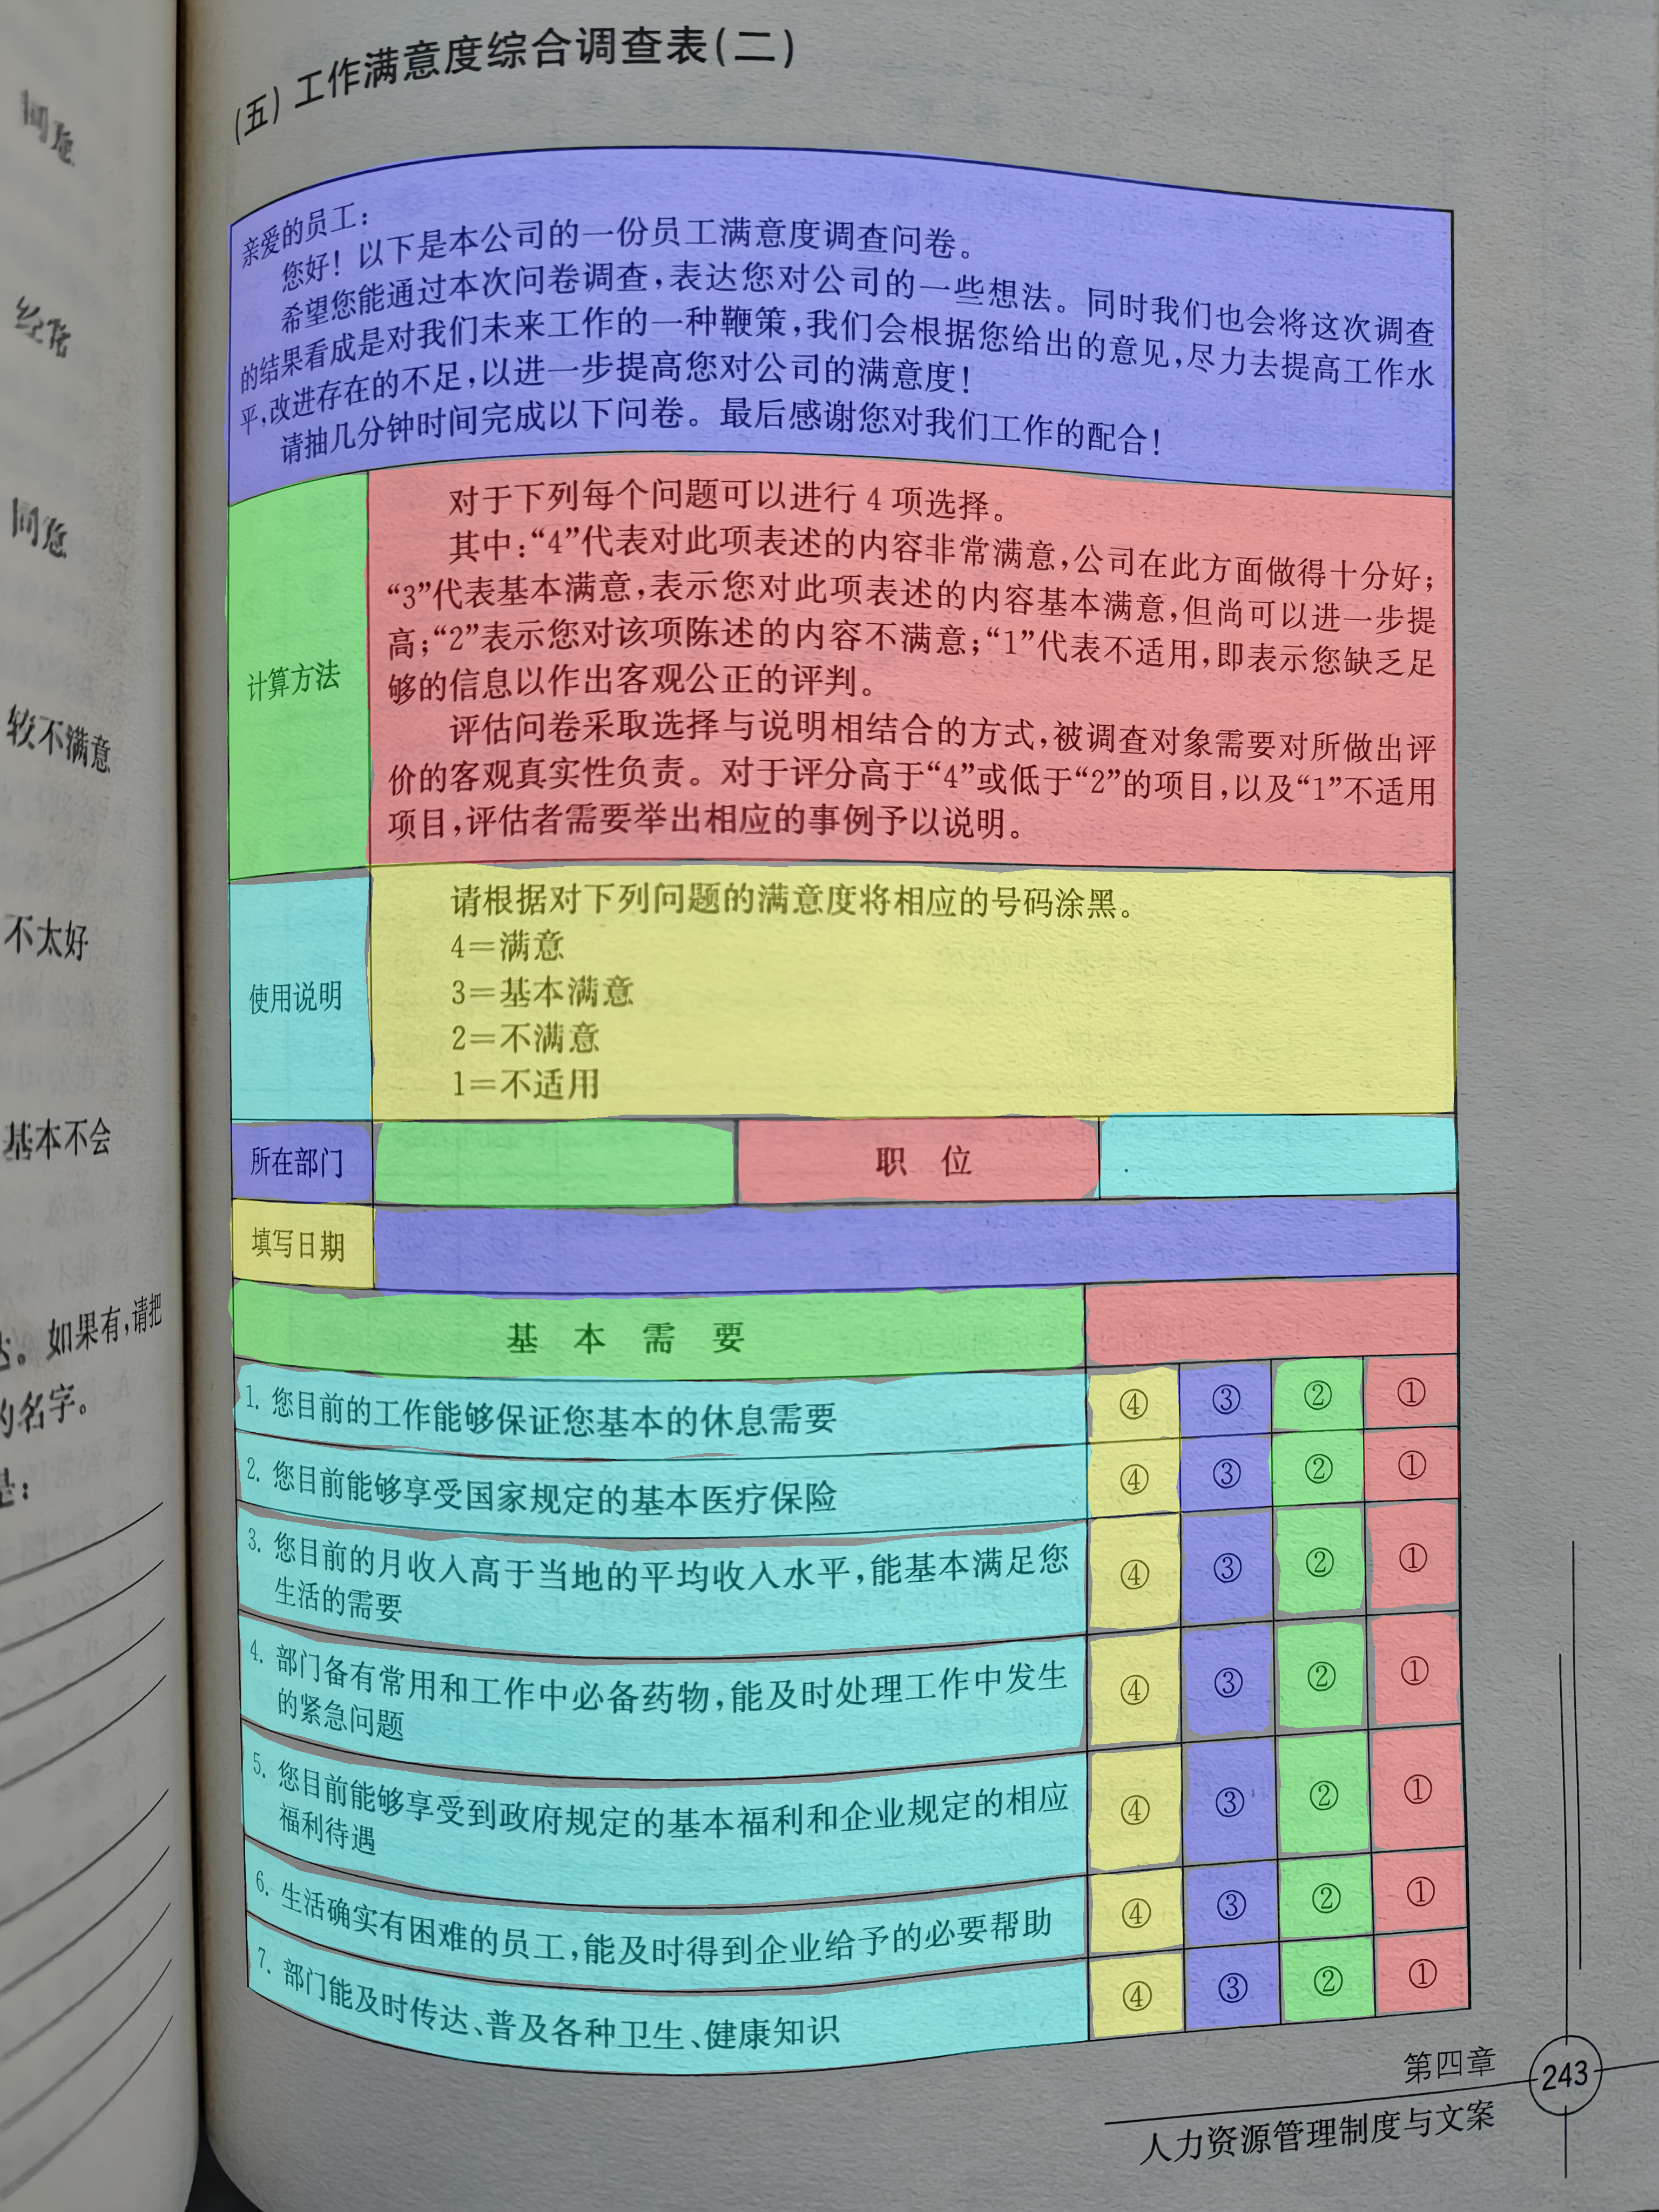
\includegraphics[width=\textwidth]{../images/vmask.png}
        \caption{原图以及掩码可视化}
    \end{subfigure}
    \hfill
    \begin{subfigure}[b]{0.45\textwidth}
        \includegraphics[width=\textwidth]{../images/local-re.jpg}
        \caption{同构表格框架图}
    \end{subfigure}
    \caption{同构表格}
    \label{fig:local-re}
\end{figure}

\section{拟解决的关键问题与创新点}
\subsection{拟解决的关键问题}

\begin{enumerate}[label=(\arabic*), leftmargin=40pt]
    \item 对表格图像提取其局部性特征和全局性特征,并将局部语义信息和全局空间依赖信息结合,以此来提高网络模型分割性能,得到一个准确的单元格分割结果。
    \item 单元格逻辑坐标定位,为后续表格结构识别提供基础,并提高表格结构识别的准确率。
\end{enumerate}
\subsection{课题的创新点}
\begin{enumerate}[label=(\arabic*), leftmargin=40pt]
    \item 基于实例分割模型,提出一种能有效分割密集且尺度不一的单元格分割算法。
    \item 根据几何学理论,为单元格逻辑定位提供了一种稳健的思路,更够有效地获取单元格的行、列以及跨行跨列的信息。
    \item 构建实例分割单元格的数据集,为模型训练提供基础,并为当前研究方向提供更加丰富的数据支持。
\end{enumerate}

\section{研究计划进度}
\noindent % 取消缩进
\textbf{第一阶段: 2024年9月 -- 2024年12月}
\begin{enumerate}[label=(\arabic*), leftmargin=40pt]
    \item 选定论文的方向,查询相关文献;
    \item 编写开题报告,介绍所要研究的具体方向和后续的安排。
\end{enumerate}
\textbf{第二阶段:2025年1月 -- 2025年3月}
\begin{enumerate}[label=(\arabic*), leftmargin=40pt]
    \item 完成总体方案、设计原理和思路设计;
    \item 完成数据集采集,初步完成数据集标注,构建算法,对图像进行训练,观察训练结果。
\end{enumerate}
\textbf{第三阶段:2025年4月 -- 2025年6月}
\begin{enumerate}[label=(\arabic*), leftmargin=40pt]
    \item 对真实文档图像样本进行标注,生成仿真文档图像样本;
    \item 改进初步构建的算法,优化算法结构,提高训练效率、准确率。
\end{enumerate}

% 参考文献部分
\section{参考文献}
\renewcommand{\section}[2]{} 
\begingroup
% 设置参考文献的格式
\fontsize{10.5pt}{12pt}\selectfont  % 设置五号字体(10.5pt)
\renewcommand{\baselinestretch}{1.0}  % 单倍行距
\setlength{\bibsep}{0pt} % 设置段前段后间距为0磅
\begin{thebibliography}{00}
    % ocr + 传统
    \bibitem{b1} Shi B, Bai X (2020). A survey on optical character recognition: Techniques, challenges, and applications[J]. International Journal of Computer Science, 28(6), 221-234. 
    % OCR技术+ 深度学习
    \bibitem{b2} Subramani N, Matton A, Greaves M, and Lam A (2020). A Survey of Deep Learning Approaches for OCR and Document Understanding[R/OL]. ArXiv, abs/2011.13534.
    % 传统算法 + 表格结构识别
    \bibitem{b3}司明. 表格识别的研究[D]. 西安科技大学, 2009.
    % 深度学习 + 表格结构是识别
    \bibitem{b4} Gilani A, R.Qasim S, Malik I, et al, Table detection using deep learning[C], in: 2017 14th IAPR international conference on document analysis and recognition (ICDAR), Vol. 1, IEEE, 2017, pp. 771–776.
    % 单元格回归结构的部分
    \bibitem{bcell} Jiang J, Simsek M, Kantarci B, and Khan S (2021). TabCellNet: Deep learning-based tabular cell structure detection[J]. Neurocomputing, 440, 12-23.
    % 研究现状、方法
    \bibitem{m1} Pyreddy P, Croft W B. TINTI: A System for Retrieval in Text Tables TITLE2:[R]. USA: University of Massachusetts, 1997.
    \bibitem{m2} Wangt Y, Phillipst I T, Haralick R. Automatic table ground truth generation and a background-analysis-based table structure extraction method[C]//Proceedings of Sixth International Conference on Document Analysis and Recognition. 2001: 528-532. https://ieeexplore.ieee.org/document/953845. doi: 10.1109/ICDAR.2001.953845.

    \bibitem{m3} Kieninger T, Dengel A. The T-Recs Table Recognition and
    Analysis System[C]//vol 1655. 1998: 255-269. doi: 10.1007/3-540-48172-9\_21.
    \bibitem{m4} Cesarini F, Marinai S, Sarti L, et al. Trainable table location
    in document images[C]//2002 International Conference on Pattern Recognition: 2002: 236-240 vol3.
    \bibitem{m5} Fan M, Kim D S. Detecting Table Region in PDF
    Documents Using Distant Supervision[M]. arXiv, 2015. http://arxiv.org/abs/1506.08891. doi: 10.48550/arXiv.1506.08891.
    \bibitem{m6} Wang Y, Hu J. A machine learning based approach for table detection on the web[C]//Proceedings of the 11th
    international conference on World Wide Web. New York, NY, USA: Association for Computing Machinery, 2002: 242-250. https://dl.acm.org/doi/10.1145/511446.511478. doi: 10.1145/511446.511478.
    \bibitem{m21} Siddiqui S A, Fateh I A, Rizvi S T R, et al. DeepTabStR: Deep Learning based Table Structure Recognition[C]//2019
    International Conference on Document Analysis and
    Recognition (ICDAR). 2019: 
    \bibitem{m22} Long R, Wang W, Xue N, et al. Parsing Table Structures in
    the Wild[M]. arXiv, 2021. http://arxiv.org/abs/2109.02199. doi: 10.48550/arXiv.2109.02199.
    \bibitem{m7} Table Recognition in Spreadsheets via a Graph Representation | IEEE Conference Publication | IEEE Xplore[EB]. https://ieeexplore.ieee.org/document/8395185.
    \bibitem{m8} Ahmed Nassar, Nikolaos Livathinos, et al. TableFormer: Table Structure Understanding with Transformers[C].Proceedings of the IEEE/CVF Conference on Computer Vision and Pattern Recognition (CVPR), 2022, pp. 4614-4623.
    \bibitem{m9} Xue W, Yu B, Wang W, et al. TGRNet: A Table Graph Reconstruction Network for Table Structure Recognition[C]//Proceedings of the IEEE/CVF International Conference on Computer Vision. 2021: 
    \bibitem{m10} Deng Y, Rosenberg D, Mann G. Challenges in End-to-End Neural Scientific Table Recognition[C]//2019 International Conference on Document Analysis and Recognition (ICDAR). 2019: 894-901. https://ieeexplore.ieee.org/document/8978078. doi: 10.1109/ICDAR.2019.00148.
    \bibitem{m11} Lee E, Kwon J, Yang H, et al. Table Structure Recognition Based on Grid Shape Graph[C]//2022 Asia-Pacific Signal and Information Processing Association Annual Summit and Conference (APSIPAASC). 2022: 1868-1873. https://ieeexplore.ieee.org/document/9980172. doi: 10.23919/APSIPAASC55919.2022.9980172.
    \bibitem{m12} Schreiber S, Agne S, Wolf I, et al. DeepDeSRT: Deep
    Learning for Detection and Structure Recognition of Tables
    in Document Images[C]//2017 14th IAPR International
    Conference on Document Analysis and Recognition
    (ICDAR): vol01. 2017: 1162-1167.
    \bibitem{m13} Agarwal M, Mondal A, Jawahar C V. CDeC-Net: Composite Deformable Cascade Network for Table Detection in Document Images[M]. arXiv, 2020. http://arxiv.org/abs/2008.10831. doi: 10.48550/arXiv.2008.10831. [80] Nazir D, Hashmi K A, Pagani A
    \bibitem{m14} Xue W, Li Q, Tao D. ReS2TIM: Reconstruct Syntactic Structures from Table Images[C]//2019 International
    Conference on Document Analysis and Recognition
    (ICDAR). 2019: 749-755. https://ieeexplore.ieee.org/document/8978027. doi: 10.1109/ICDAR.2019.00125.
    \bibitem{m15} Tensmeyer C, Morariu V I, Price B, et al. Deep Splitting and
    Merging for Table Structure Decomposition[C]//2019
    International Conference on Document Analysis and
    Recognition (ICDAR). 2019: 114-121. https://ieeexplore.ieee.org/document/8977975. doi: 10.1109/ICDAR.2019.00027.
    \bibitem{m16} Deng Y, Rosenberg D, Mann G. Challenges in End-to-End Neural Scientific Table Recognition[C]//2019 International Conference on Document Analysis and Recognition (ICDAR). 2019: 894-901. https://ieeexplore.ieee.org/document/8978078. doi: 10.1109/ICDAR.2019.00148.
    \bibitem{m17} Paliwal S, D V, Rahul R, et al. TableNet: Deep Learning model for end-to-end Table detection and Tabular data
    extraction from Scanned Document Images[M]. arXiv, 2020. http://arxiv.org/abs/2001.01469. doi: 10.48550/arXiv.2001.01469.
    \bibitem{m18} Prasad D, Gadpal A, Kapadni K, et al. CascadeTabNet: An approach for end to end table detection and structure recognition from image-based documents[M]. arXiv, 2020. http://arxiv.org/abs/2004.12629. doi: 10.48550/arXiv.2004.12629.
    \bibitem{m19} Nazir D, Hashmi K A, Pagani A, et al. HybridTabNet: Towards Better Table Detection in Scanned Document Images[J]. Applied Sciences, 2021, 11(18): 8396. doi: 10.3390/app11188396.
    \bibitem{m20} Hashmi K A, Pagani A, Liwicki M, et al. CasTabDetectoRS: Cascade Network for Table Detection in Document Images with Recursive Feature Pyramid and Switchable Atrous Convolution[J]. Journal of Imaging, 2021, 7(10): 214. doi: 10.3390/jimaging7100214.
    \bibitem{m23} Xing H, Gao F, Long R, et al. LORE: Logical Location Regression Network for Table Structure Recognition[M]. arXiv, 2023. http://arxiv.org/abs/2303.03730. doi: 10.48550/arXiv.2303.03730.
    \bibitem{m24} Chandran S, Kasturi R. Structural recognition of tabulated data[C]//Proceedings of 2nd International Conference on Document Analysis and Recognition (ICDAR ’93). 1993: 516-519. https://ieeexplore.ieee.org/document/395683. doi: 10.1109/ICDAR.1993.395683.
    \bibitem{m25}  Göbel M, Hassan T, Oro E, et al. ICDAR 2013 Table Competition[C]//2013 12th International Conference on Document Analysis and Recognition. 2013: 1449-1453.
    \bibitem{m26} Oro E, Ruffolo M. PDF-TREX: An Approach for Recognizing and Extracting Tables from PDF Documents[C]//2009 10th International Conference on Document Analysis and Recognition. 2009: 906-910. https://ieeexplore.ieee.org/document/5277546/footnotes\#footnotes.



    % \bibitem{data1} Fang J, Tao X, Tang Z, et al. Dataset, Ground-Truth and
    % Performance Metrics for Table Detection Evaluation[J]. Proceedings - 10th IAPR International Workshop on Document Analysis Systems, DAS 2012, 2012. doi: 10.1109/DAS.2012.29.
    % \bibitem{data2} Göbel M, Hassan T, Oro E, et al. ICDAR 2013 Table Competition[C]//2013 12th International Conference on Document Analysis and Recognition. 2013: 1449-1453.
    % \bibitem{data3} Gao L, Yi X, Jiang Z, et al. ICDAR2017 Competition on Page Object Detection[C]//2017 14th IAPR International
    % Conference on Document Analysis and Recognition
    % (ICDAR): vol 01. 2017: 1417-1422.
    % \bibitem{data4} Gao L, Huang Y, Déjean H, et al. ICDAR 2019 Competition
    % on Table Detection and Recognition (cTDaR)[C]//2019
    % International Conference on Document Analysis and
    % Recognition (ICDAR). 2019: 1510-1515. https://ieeexplore.ieee.org/document/8978120. doi: 10.1109/ICDAR.2019.00243.
    % \bibitem{data5} N. Siegel, N. Lourie, R. Power, et al. Extracting scientific figures with distantly supervised neural networks, in: Proceedings of the 18th ACM/IEEE on joint conference on
    % digital libraries, 2018, pp. 223–232.
    % \bibitem{data6} Zhong X, ShafieiBavani E, Yepes A J. Image-based table
    % recognition: data, model, and evaluation[M]. arXiv, 2020. http://arxiv.org/abs/1911.10683. doi: 10.48550/arXiv.1911.10683.
    % \bibitem{data7} Li M, Cui L, Huang S, et al. TableBank: A Benchmark
    % Dataset for Table Detection and Recognition[EB]//arXiv.org. (2019-03-05). https://arxiv.org/abs/1903.01949v2.
    % \bibitem{data8} Chi Z, Huang H, Xu H D, et al. Complicated Table Structure Recognition[M]. arXiv, 2019. http://arxiv.org/abs/1908.04729. doi: 10.48550/arXiv.1908.04729.
    % \bibitem{data9} Zheng X, Burdick D, Popa L, et al. Global Table Extractor
    % (GTE): A Framework for Joint Table Identification and Cell
    % Structure Recognition Using Visual Context[M]. arXiv,2020. http://arxiv.org/abs/2005.00589. doi: 10.48550/arXiv.2005.00589.
    % \bibitem{data10} Long, R, Wang, W, Xue, N, Gao, F, Yang, Z, Wang, Y, Xia, G (2021). Parsing Table Structures in the Wild. 2021 IEEE/CVF International Conference on Computer Vision (ICCV), 924-932.
    % \bibitem{data11} Smock B, Pesala R, Abraham R. PubTables-1M: Towards comprehensive table extraction from unstructured
    % documents[M]. arXiv, 2021. http://arxiv.org/abs/2110.00061. doi: 10.48550/arXiv.2110.00061
    % \bibitem{data12} Zhong X, ShafieiBavani E, Yepes A J. Image-based table
    % recognition: data, model, and evaluation[M]. arXiv, 2020. http://arxiv.org/abs/1911.10683. doi: 10.48550/arXiv.1911.10683.
    % \bibitem{data13} Ly N T, Takasu A, Nguyen P, et al. Rethinking Image-based
    % Table Recognition Using Weakly Supervised
    % Methods[C]//Proceedings of the 12th International
    % Conference on Pattern Recognition Applications and
    % Methods. 2023: 872-880. http://arxiv.org/abs/2303.07641. doi: 10.5220/0011682600003411.
    
    % \bibitem{b6} Dosovitskiy, Alexey, et al. "An image is worth 16x16 words: Transformers for image recognition at scale." arXiv preprint arXiv:2010.11929 (2020).
    % \bibitem{b7} Bing S ,Tao G ,Hongbo S , et al. Quality-related process monitoring scheme based on neighborhood embedding canonical correlation analysis model[J]. Journal of the Taiwan Institute of Chemical Engineers,2023,152.
    % \bibitem{b8} Minqiang Y ,Yushan W ,Yongfeng T , et al. Trial Selection Tensor Canonical Correlation Analysis (TSTCCA) for Depression Recognition with Facial Expression and Pupil Diameter.[J]. IEEE journal of biomedical and health informatics,2023,PP.
    % \bibitem{b9} Lijia L ,Weida W ,Shiyi B , et al. Robust and sparse canonical correlation analysis for fault detection and diagnosis using training data with outliers[J]. Expert Systems With Applications,2024,236.
    % \bibitem{b10} Jiali Y . Application of improved BP neural network model in bank financial accounting[J]. Intelligent Systems with Applications,2022,16.
\end{thebibliography}
\endgroup


{
    
\newpage
\newgeometry{left=3.18cm,right=3.18cm,top=2.54cm, bottom=2.54cm}
\thispagestyle{empty}
\begin{center}
     {\huge 学位论文原创性声明}
\end{center}

\vspace*{3\baselineskip}

\begin{spacing}{2}
\zihao{4}
郑重声明:所呈交的学位论文《基于YOLOv7和目标跟踪的人流量检测系统》,是本
人在导师的指导下,独立进行研究取得的成果。除文中已经注明引用
的内容外,本论文不包含其他个人或集体已经发表或撰写过的作品、
研究成果。对本文的研究做出贡献的个人和集体,均已在文中以明确
方式标明。本人完全意识到本声明的法律后果,并承诺因本声明而产
生的的法律结果由本人承担。
\end{spacing}

\vspace*{5\baselineskip}

\zihao{4} 学位论文作者:罗小龙

\vspace*{2\baselineskip}

\zihao{4} 日期:2023 年 5 月 19 日

}
% \end{sloppypar}
\end{document}

